\documentclass{beamer}
\usetheme{VATT}
\usepackage[utf8]{inputenc}

\usepackage{todonotes}
\presetkeys{todonotes}{inline}{}


\title{team meeting}
\author{jjycavailles }
\date{June 2019}

\usepackage{natbib}
\usepackage{graphicx}


%\begin{center}
%  
\includegraphics[width = 25mm]{LogoInsa.png} \hfill
%  
\includegraphics[width = 30mm]{logo_cnrs.jpg}
%\end{center}

%\titlegraphic{
\includegraphics[width=2cm]{cnrs.png}}
\title{Destabilizing effects of controlling ecosystem behavior}




%\subtitle{Projet 4GMM}
%\author{VATT Communication}
\author[Jérôme Cavaillès, Yuval Zelnik]{%
  \texorpdfstring{%
    \begin{columns}
      \column{.33\linewidth}
      \centering
      \it{Jérôme Cavaillès} \\ INSA Toulouse \\ Paul Sabatier
      \column{.33\linewidth}
      \centering
     Supervisor \\ \it{Yuval Zelnik} \\ \it{Michel Loreau}
     % \column{.33\linewidth}
     % \centering
     % Author 3 \\ Institute 3
    \end{columns}
 }
 {Author 1, Author 2, Author 3}
}
\date{\today}
\institute{%
  \texorpdfstring{%
    \begin{columns}
      \column{.9\linewidth}
      \centering
   %   \url{lcaselle@etud.insa-toulouse.fr} \\
    %  \url{jcavaill@etud.insa-toulouse.fr} \\
      %\url{firstname.lastname@institute3.com}
    \end{columns}
 }
 {Author 1, Author 2, Author 3}
}



\begin{document}


\begin{frame}[plain,t]
\titlepage
% add logo sur la page de présentation
\end{frame}



\begin{frame}
\frametitle{Contents} 
%\todo{content before of after context ?}
\tableofcontents
\end{frame}



\section{Context}

\begin{frame}
\frametitle{Context} % PRESENT IN 2 COLUMNS ?
\begin{enumerate}
\item Overall goal : protect ecosystem
\begin{itemize}
    \item protect services of a forest (ex : wood production)
\end{itemize}
\item[]
%$\Rightarrow$ 
\item Stabilize ecosystem 
\begin{itemize}
    \item wildfire reduction
\end{itemize}
\item[]
\item Long term consequences 
\begin{itemize}
    \item dead wood accumulation
\end{itemize}
\item[]
\item In some cases : collapse of the system 
\begin{itemize}
    \item more damaging fire
\end{itemize}
\end{enumerate}
\end{frame}




\section{Methods}

\subsection{Model}
\begin{frame}
\frametitle{Model}
\[
\left\{
\begin{array}{rcl}
\frac{dN}{dt} & = & gN(1-N/K)(N/A-1) + \delta_F(t)s(t)(N+\alpha W)\\
\\
\frac{dW}{dt} & = & \mu N-dW  + \delta_F(t)s(t)\beta(N+\alpha W)\\
\end{array}
\right.
\]
\begin{itemize}
    \item N : living biomass
    \item W : death biomass
\end{itemize}
\end{frame}


\begin{frame}
\frametitle{Non-dimensionalisation Model}
\begin{itemize}
    \item we adimensionalise the system
    \item 7 parameters remains
    \item Adimensionalised system : 
    \[
\left\{
\begin{array}{rcl}
\frac{dN}{dt} & = & N(1-N)(N-a) + \delta_F(t)s(t)(N+\alpha W)\\
\\
\frac{dW}{dt} & = & mN-dW  + \delta_F(t)s(t)\beta(N+\alpha W)\\
\end{array}
\right.
\]

\end{itemize}
\end{frame}


% PRESENT "TIMES SERIES" HERE OTHERWISE MEASURES IS MORE DIFFICULT TO UNDERSTAND
\begin{frame}
\frametitle{Time series}
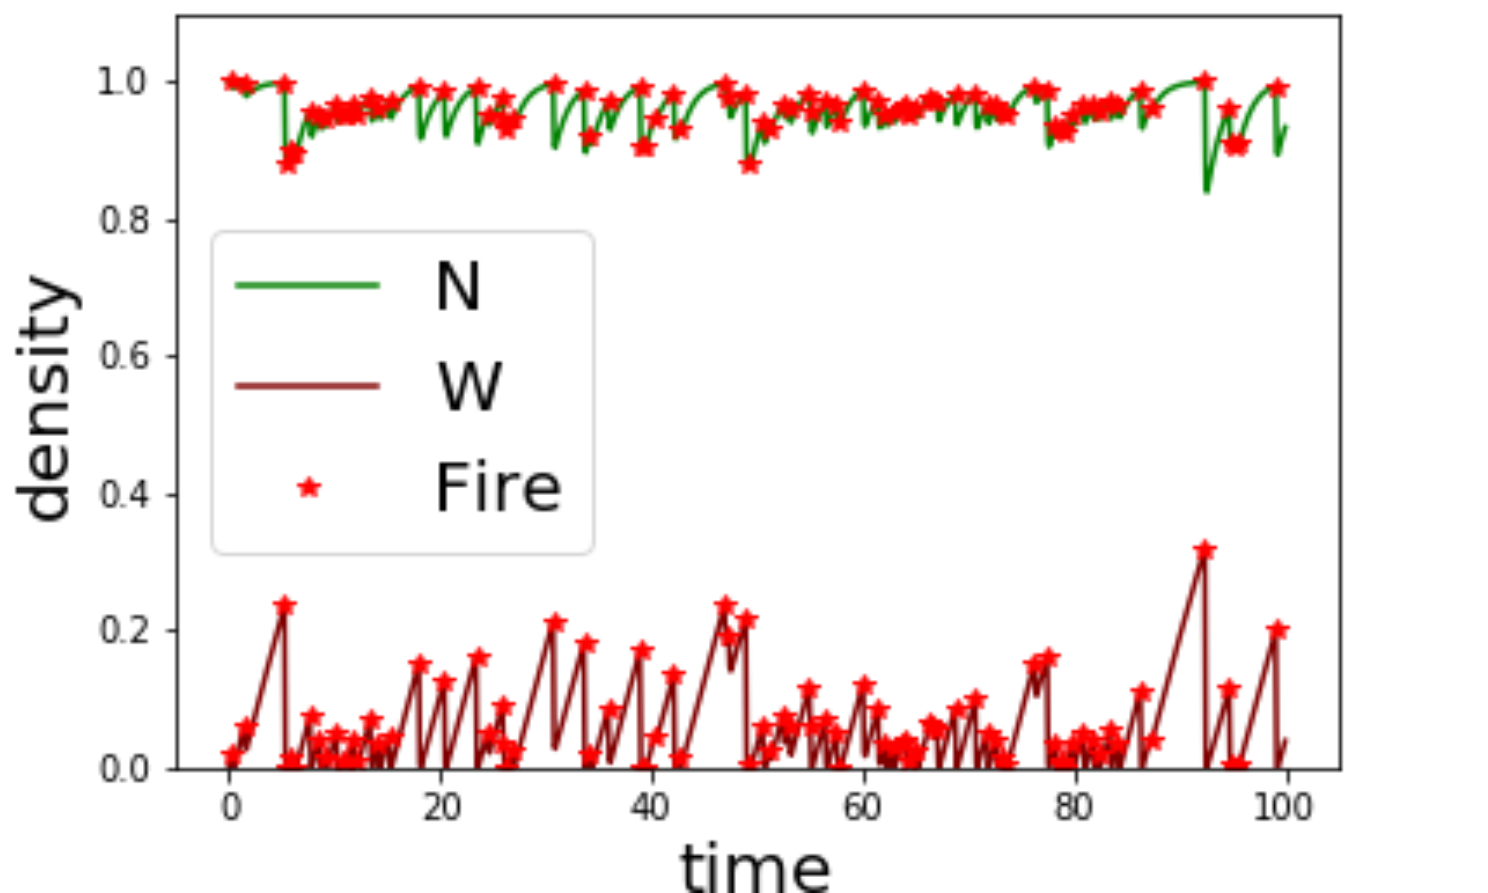
\includegraphics[width=10.cm]{time_series.png}
%\todo{EXPLAIN THE DYNAMICS}
\end{frame}


\subsection{Measures}
\begin{frame}
\frametitle{Measures}

\begin{itemize}
    \item Variability
    % forest management, especially few years ago, tend to lock the dynamics of the forest, to keep the same biomass density.  The explanation is, among other, to regularise the wood production or to protect forest from fire).  This management can be characterise by the will to reduce variability.
    \begin{itemize}
        \item Variance between 10\% and 20\% of the time study
        \item Measure before a collapse to avoid biais
    \end{itemize}
    \item Collapse probability
    \begin{itemize}
        \item average collapse for several simulations
    \end{itemize}
\end{itemize}

%\begin{itemize}
 %   \item Define variability
  %  \item problem with the computation of variability
   % \item Define collapse probability
    %\item problem with the computation of collapse probability
%\end{itemize}

\end{frame}


\section{Results}




\begin{frame}
\frametitle{Frequency impacts}
%\todo{loop : variability VS collapse probability}
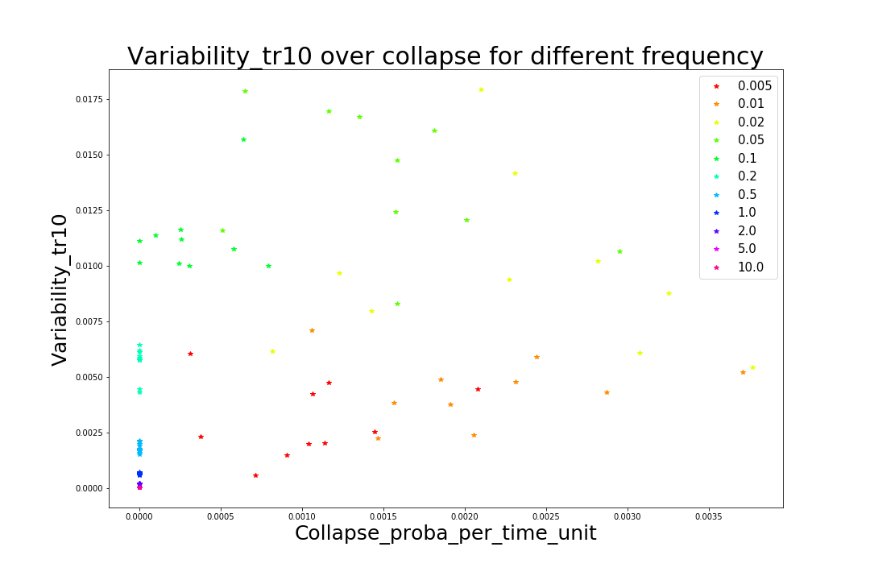
\includegraphics[width=9.cm]{loop.png}
\end{frame}


\begin{frame}
\frametitle{Study of the peaks}
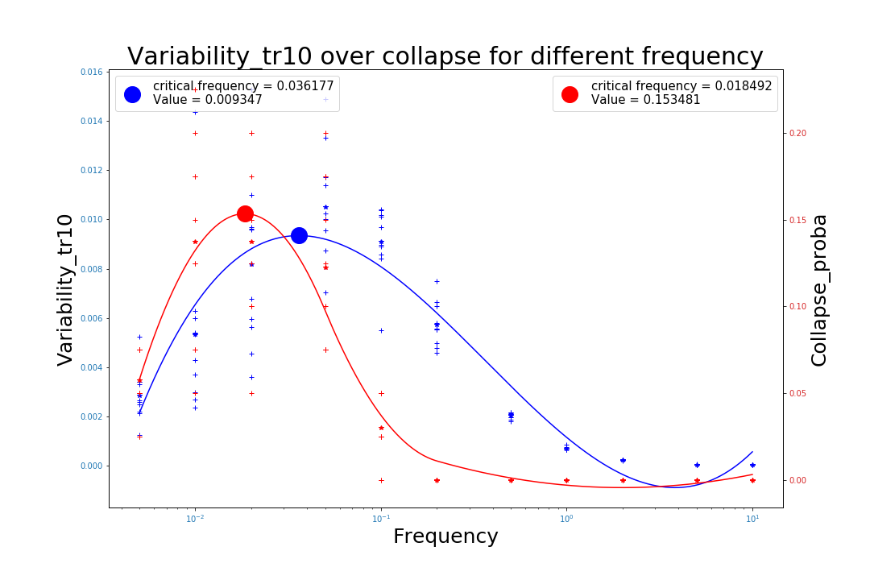
\includegraphics[width=9.cm]{2_peaks.png}
\end{frame}


\begin{frame}
\frametitle{Another approach}
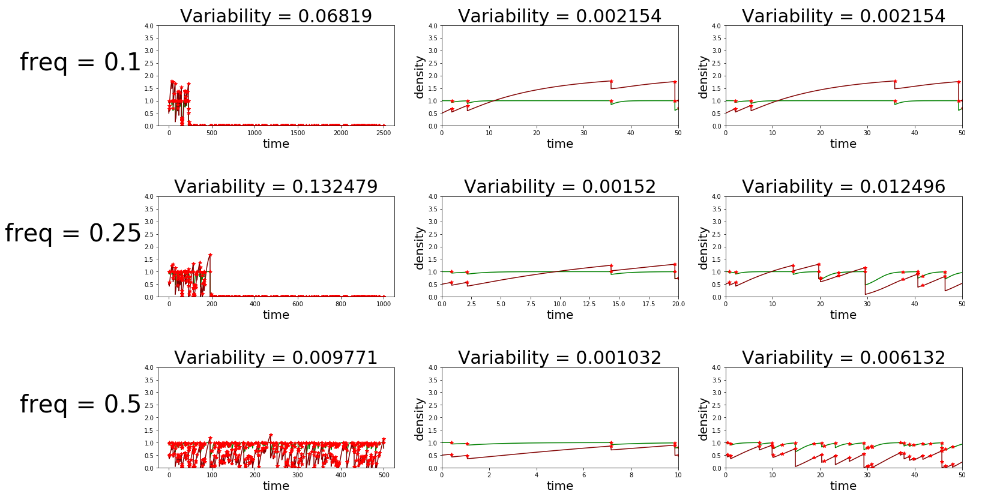
\includegraphics[width=9.cm]{same_fire.png}
\end{frame}


\begin{frame}
%\frametitle{}
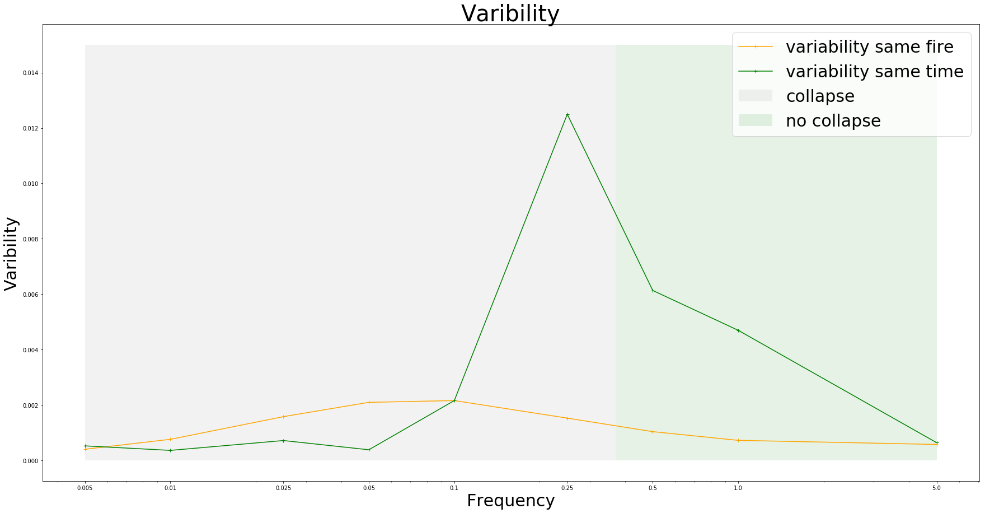
\includegraphics[width=9.cm]{variability.png}
\end{frame}


\section{Conclusion}

\subsection{Synthesis}
\begin{frame}
\frametitle{Synthesis}
useful ?
\end{frame}


\subsection{Opening}
\begin{frame}
\frametitle{Opening}
%\todo{list of what I am going to do after}
\begin{enumerate}
    \item Explore exhaustively the various scenarios
    \item How the shape of the loop could changed ? %\todo{reformulate}
    \item Why the shape of the loop could changed ? %\todo{reformulate}
\end{enumerate}

\end{frame}




\begin{frame}
\frametitle{References}
\bibliographystyle{plain}
\bibliography{references}
\end{frame}


\begin{frame}

\begin{center}
Thank you for your attention.
\\
Have you any questions ?
\end{center}

\end{frame}



\end{document}
